\label{chap:results}

In this chapter we will cover the results obtained with this algorithm and
other similar software and analyze how well it performs when compared to
classic solutions. The algorithm was tested on a set of graphs consisting of 
10, 100, 1000, 10000 and 100000 nodes each. In order to assert its efficiency, 
the same graphs were drawn with other available open-source software: the Graphviz
dot library \cite{gansner2009drawing} and the Eclipse Java GEF library \cite{rubel2011eclipse}.

\subsection{Placing Performance}

The main performance concerns for this algorithms were mainly related to the 
time necessary to place the graph according to the given restrictions. Since 
both Graphiz dot and GEF do not have rules based placing, they rely on 
traditional methods such as grid or tree layout, the actual layout time of our 
implementation is slower. However, due to the nature of genetic algorithms, we 
do not necessarily have to stop once a population which meets all the criteria 
has been found. A user can easily specify after how many steps the algorithm may 
stop, and the result will be a layout which is an approximation of the ideal one.

\subsection{Routing Performance}

When it comes to small data models (graphs), the proposed orthogonal routing 
solution varies in time needed to route the connections. It can go from being 
faster than the other software to being approximately 10-15 percent slower than 
classical shortest path or manhattan distance based grid solutions, depending on 
the complexity of the model and its connections. This is mainly because of the 
restriction imposed on routes not crossing each other. However, once we reach 
bigger graphs, the ones containing over 10000 nodes, the solution is smoother and
scales better, mainly because everything is already placed correctly and connections 
are shorter and do not have to go around too many elements.

\begin{figure}[ht] \centering
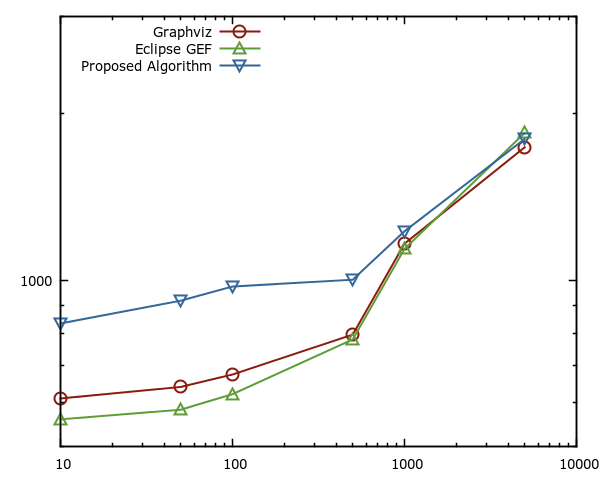
\includegraphics[width=0.5\textwidth]{src/under_10000.png}
\caption{Performance graph for tests containing under 10000} \end{figure}

\begin{figure}[ht] \centering
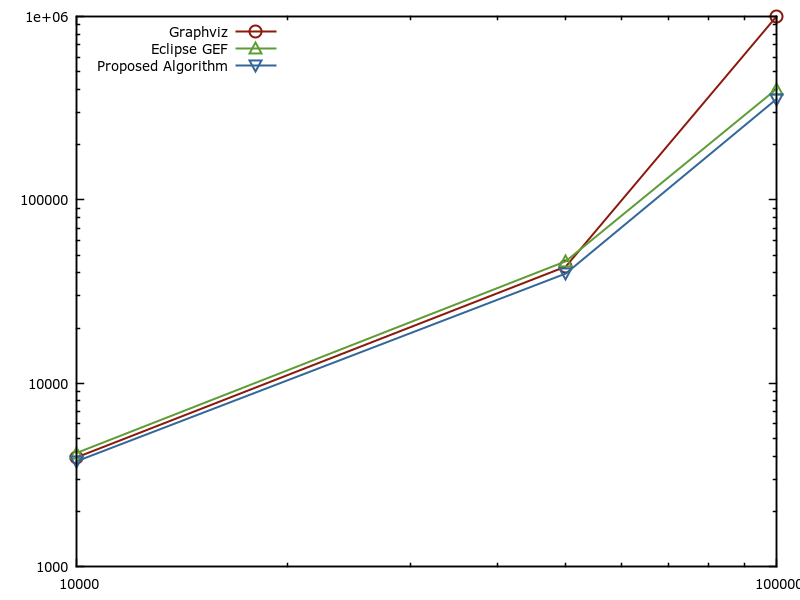
\includegraphics[width=0.5\textwidth]{src/over_10000.png}
\caption{Performance graph for tests containing over 10000} \end{figure}
